\FloatBarrier
\begin{figure}[!h]
\begin{subfigure}[t]{0.5\textwidth}
	\centering
	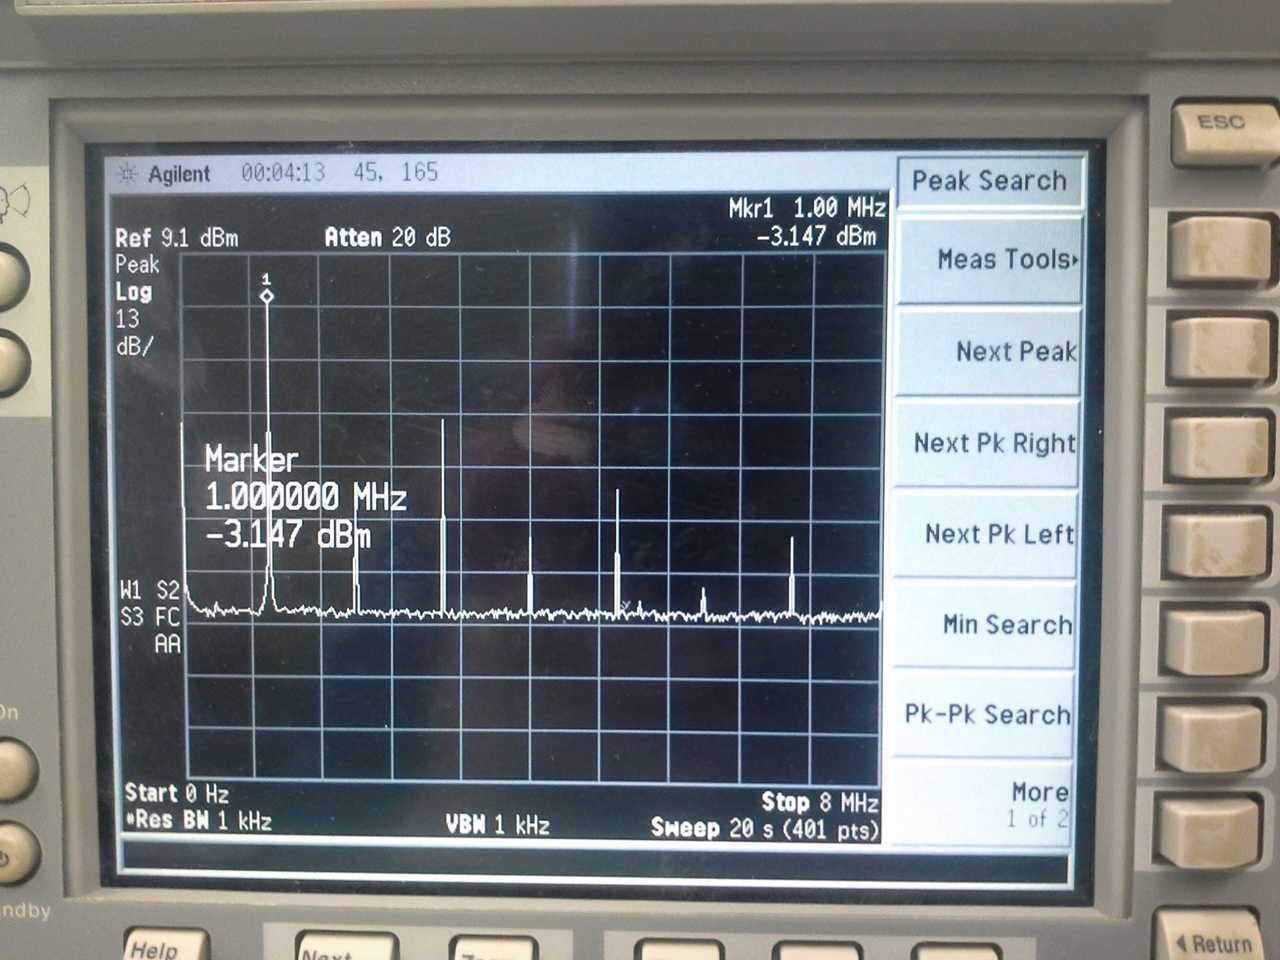
\includegraphics[scale=0.17]{../Grafiken/TraegerspannungOberwellen_0.jpg}
	\caption{Grundschwingung \label{fig:traegerspannungoberwellen_0}}
\end{subfigure}%
~
\begin{subfigure}[t]{0.5\textwidth}
	\centering
	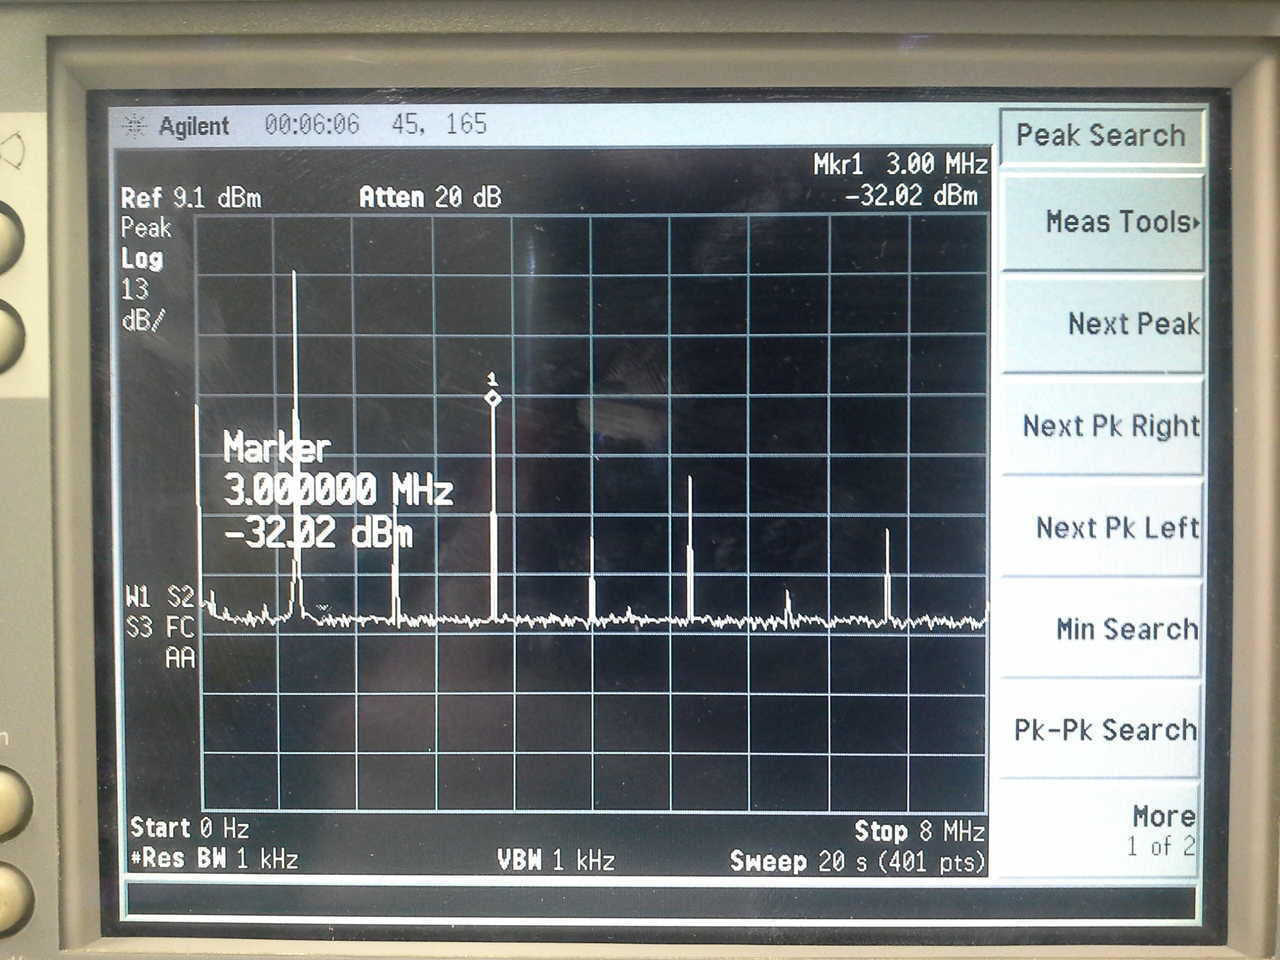
\includegraphics[scale=0.17]{../Grafiken/TraegerspannungOberwellen_2.jpg}
	\caption{Zweite Oberschwingung\label{fig:traegerspannungoberwellen_2}}
\end{subfigure}
	\caption{Frequenzspektrum der verwendeten Trägerspannung. Zu erkennen sind die Oberschwingungen,
		     die bereits in der ursprünglichen Spannung vorhanden sind. \label{fig:traegerspannungoberwellen}}
\end{figure}
\FloatBarrier